\let\negmedspace\undefined
\let\negthickspace\undefined
\documentclass[journal]{IEEEtran}
\usepackage[a5paper, margin=10mm, onecolumn]{geometry}
%\usepackage{lmodern} % Ensure lmodern is loaded for pdflatex
\usepackage{tfrupee} % Include tfrupee package

\setlength{\headheight}{1cm} % Set the height of the header box
\setlength{\headsep}{0mm}     % Set the distance between the header box and the top of the text

\usepackage{gvv-book}
\usepackage{gvv}
\usepackage{cite}
\usepackage{amsmath,amssymb,amsfonts,amsthm}
\usepackage{algorithmic}
\usepackage{graphicx}
\usepackage{textcomp}
\usepackage{xcolor}
\usepackage{txfonts}
\usepackage{listings}
\usepackage{enumitem}
\usepackage{mathtools}
\usepackage{gensymb}
\usepackage{comment}
\usepackage[breaklinks=true]{hyperref}
\usepackage{tkz-euclide} 
\usepackage{listings}
% \usepackage{gvv}                                        
\def\inputGnumericTable{}                                 
\usepackage[latin1]{inputenc}                                
\usepackage{color}                                            
\usepackage{array}                                            
\usepackage{longtable}                                       
\usepackage{calc}                                             
\usepackage{multirow}                                         
\usepackage{hhline}                                           
\usepackage{ifthen}                                           
\usepackage{lscape}
\begin{document}

\bibliographystyle{IEEEtran}
\vspace{3cm}

\title{9.1.2}
\author{EE24BTECH11001 - Aditya Tripathy}
 \maketitle
% \newpage
% \bigskip
{\let\newpage\relax\maketitle}

\renewcommand{\thefigure}{\theenumi}
\renewcommand{\thetable}{\theenumi}
\setlength{\intextsep}{10pt} % Space between text and floats


\numberwithin{equation}{enumi}
\numberwithin{figure}{enumi}
\renewcommand{\thetable}{\theenumi}


\textbf{Question}:\\
Plot a solution to the following differential equation:\\
    $y^\prime + 5y = 0$
\\
\textbf{Solution: }\\
The aim is to find the difference equation using the trapezoidal law using the following initial conditions,
$x_0 = 0, y_0 = 1$\\

\begin{align}
    y^{\prime} &= -5y \\
    \int_{y_n}^{y_{n+1}} \, dy &= \int_{x_n}^{x_{n+1}} -5y \, dx\\
\end{align}
Using the trapezoidal rule,
\begin{align}
    J &= \int_a^b f\brak{x}\, dx\\
    &\approx h\brak{\frac{1}{2}f\brak{x} + f\brak{x_1} + f\brak{x_2} \cdots + f\brak{x_{n-1}} + \frac{1}{2}f\brak{b}}\\
    \frac{y_{n+1} - y_n}{1}\brak{\frac{1}{2} + \frac{1}{2}}
    &= -5\frac{x_{n+1} - x_{n}}{1}\brak{\frac{y_n}{2} +\frac{y_{n+1}}{2}} \\ 
    \xrightarrow{} y_{n+1} &= \frac{\brak{2-5h}y_n}{5h+2} 
\end{align}
Another way we can arrive at the differnce equation is by using the Bilinear transform,\\
Applying Laplace Transform to both sides of the differential equation,
\begin{align}
    sY - sy_0 + 5Y &= 0\\
    Y\brak{s} &= \frac{sy_0}{s+5}\\
\end{align}
    \text{Apply Bilinear Transform, with T = h}\\
\begin{align}
    s &= \frac{2}{T} \frac{1-z^{-1}}{1+z^{-1}}\\
    Y\brak{z} &= \frac{2y_0\brak{1 - z^{-1}}}{2\brak{1 - z^{-1}} + 5h\brak{1 + z^{-1}}}\\
    Y\brak{z} &= \frac{2y_0\brak{1 - z^{-1}}}{\brak{2+5h} + \brak{5h-2}z^{-1}}\\
    \alpha &= -\frac{5h-2}{5h+2}\\
    Y &= \frac{2y_0}{5h+2}\brak{\frac{1}{1- \alpha z^{-1}} - \frac{z^{-1}}{1 - \alpha z^{-1}}}\\
    \brak{1 -\alpha z^{-1}}Y &= \frac{2y_0}{5h+2}\brak{1-z^{-1}}
\end{align}
Applying inverse Z-transform,
\begin{align}
    y_n - y_{n-1} &=   \frac{2y_0}{5h+2}\brak{\delta \sbrak{n} - \delta \sbrak{n-1}}\\
\end{align}
To check how close the approximate graph is to the actual solution, we will solve the original 
equation using a Laplace Transform method:\\
Let $\mathcal{L}\brak{y} = Y$\\
\begin{align}
    \brak{sY - y_0} +5Y = 0\\
    \brak{s + 5}Y = y_0\\
    Y = \frac{1}{s + 5}\\
\end{align}
    \text{Substituting $y_0 = 1$},\\
\begin{align}
    Y = \frac{1}{s + 5}\\
\end{align}
    \text{Now, we take the inverse laplace transform to get a solution,}\\
\begin{align}
    \mathcal{L}^{-1}\brak{\frac{1}{s+5}} = e^{-5x}u\brak{x}
\end{align}
For the following approximate graph, I chose $h = 0.01$ and $h = 0.1$.
\begin{figure}[h!]
   \centering
   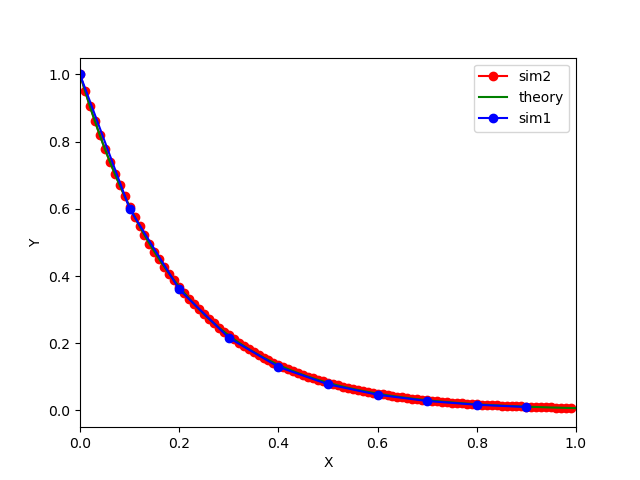
\includegraphics[width=0.7\columnwidth]{figs/fig.png}
    \caption{Approximate solution of the DE}
\end{figure}
\end{document}  
